% LaTeX resume using res.cls
\documentclass[line,margin]{res}
%\usepackage{helvetica} % uses helvetica postscript font (download helvetica.sty)
%\usepackage{newcent}   % uses new century schoolbook postscript font

\newcommand{\zh}{Z\"{u}rich}
\usepackage{charter}
\usepackage{graphicx}
\usepackage{wrapfig}
\usepackage[super]{nth}
\usepackage[utf8]{inputenc}

\begin{document}

\name{Eivind Fonn}
% \address used twice to have two lines of address
\address{Høgreina 394, NO-7079 Flatåsen}
\address{+41 41 44 98 89, evfonn@gmail.com}


\begin{resume}

\section{PERSONALIA}

\begin{wrapfigure}{R}{0.13\textwidth}
  \vspace{-0.6cm}
  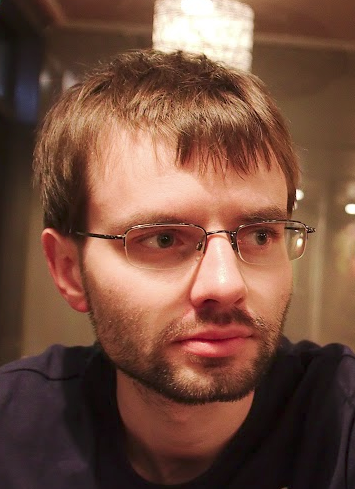
\includegraphics[width=1.5cm]{photo.png}
\end{wrapfigure}

I am a 31 year old Norwegian, born, grown up and with undergraduate studies in
Trondheim, Norway. Moved to Zürich, Switzerland for graduate studies. Interested
in mathematics, computing, programming, photography, chess and books.

\section{EDUCATION}

{\em Ph.D.}, computational science \hfill 2009-09 $\to$ 2013-11 \\
ETH \zh, \zh, Switzerland \\
Solving high-dimensional kinetic transport equations, bridging the ``curse of
dimensionality''. Particular focus on Shearlet frames and the Boltzmann equation.

{\em Master of Technology}, industrial mathematics \hfill 2004-08 $\to$ 2009-06 \\
NTNU, Trondheim, Norway \\
Specialisation in numerical analysis and differential geometry.

\section{EXPERIENCE}

{\em Research Scientist} \hfill 2014-05 $\to$ present \\
SINTEF Applied Mathematics, Trondheim, Norway \\
A variety of projects (see below), mostly large-scale parallel simulations using
isogeometric analysis finite element methods.

{\em Associate professor} \hfill 2016-01 $\to$ 2016-06 \\
NTNU, Trondheim, Norway \\
Part-time faculty position, lecturer of the TMA4280 \emph{Introduction to
  Supercomputing} course.

{\em Ph.D. student} \hfill 2009-09 $\to$ 2013-11 \\
ETH \zh, \zh, Switzerland \\
Solving high-dimensional kinetic transport equations, bridging the ``curse of
dimensionality''. Implementation in Matlab and Python. Includes a 40\% teaching
load.

{\em Software engineer} \hfill Summer 2009 \\
Jeeves, Trondheim, Norway \\
Implemented a translation tool built on Google Translate, which can read and
write a number of different formats (such as Microsoft Word and database
tables), with some facilities for correcting erroneous translations and
learning.

{\em Software engineer} \hfill Summer 2008 \\
Yahoo! Technologies, Trondheim, Norway \\
Implemented an adapter between MySQL and Yahoo's internal vertical search
platform Vespa, together with several demo cases. Responsibilities included the
entire process, from design to completion.

% {\em Scientific assistant} \hfill Summer 2007 \\
% ETH \zh, \zh, Switzerland \\
% Implemented a finite volume method for solving the convection/diffusion/reaction
% equation in Matlab. Also did some post-processing of photonic crystal
% simulations. This was an IAESTE internship.

\section{SKILLS}

\begin{itemize}
\item {\em Programming languages:} I am an expert in Python, and I am proficient
  in C, C++ and Matlab, and some lisp dialects. I have experience with Java,
  C$\sharp$, PHP and Javascript, although this can be 5 to 10 years old. I
  dabble in Haskell and Rust.
\item {\em Databases:} PostgreSQL when possible, MySQL when necessary.
\item {\em Other:} I have a decade of experience running Linux distributions for
  personal use, and I have administered several servers.
\item {\em Languages:} Fluent Norwegian and English, reasonable German.
\end{itemize}

\section{AWARDS}

\begin{itemize}
\item Winnie and Ragnar Mathisen's award for best student of technology
  or architecture in the 2009 graduating class at NTNU.
\item The Norwegian Computing Centre's award for best master thesis in
  mathematics or ICT at NTNU in 2008/09.
\item The Stubban award for the most promising master candidate in
  mathematics at NTNU among the 2009 graduating class.
\end{itemize}

\section{ASSORTED}

\begin{itemize}
\item Part organiser of the inaugural edition of KoMiN---a now annual conference
  for mathematics students in Norway.
\item Designed problems, graded answers and maintained the website for the Abel
  Competition, the Norwegian mathematical olympiad for high school students.
\item Driving force and main organiser of the first two editions of the
  Norwegian Rubik's Cube Championship.
\item Former national record holder in Rubik's Cube speedsolving and
  speedsolving while blindfolded (single and multiple).
\end{itemize}

\section{POSITIONS OF TRUST}

\begin{itemize}
\item Webmaster\footnote{{\tt http://iaeste.ch/}} and board member for the
  IAESTE Local Comittee \zh\ for four years (2010-2013).
\item Recognised by the World Cubing Association as a competition delegate.
\item Webmaster and board member for the Student association Nabla\footnote{{\tt
    http://nabla.no}} at NTNU for three years (2005-2007).
\end{itemize}

% \section{REFERENCES}

% On request.

% \begin{itemize}
% \item Prof. Dr. Ralf Hiptmair, Seminar for Applied Mathematics, ETH Zurich \\
%   +41 44 632 34 04, ralf.hitpmair@sam.math.ethz.ch
% \item Prof. Dr. Philipp Grohs, Seminar for Applied Mathematics, ETH Zurich \\
%   +41 44 632 32 00, philipp.grohs@sam.math.ethz.ch
% \end{itemize}

\section{SOCIAL SITES}

\begin{itemize}
\item Github: \texttt{http://github.com/TheBB}
\item LinkedIn: \texttt{http://www.linkedin.com/pub/eivind-fonn/5/364/67}
\end{itemize}

\section{PROJECTS}

{\em eSushi: Prediction and optimization of fish hauls}
\hfill 2016-06 $\to$ 2016-08 \\
{\small Partners: SINTEF, a coalition of seafood companies} \\
This project aims to predict fish distribution in the Norwegian and Barents sea
to optimize catch rates for the fishing industry.
\begin{itemize}
\item Performed preliminary statistical analysis (Gaussian processes) to
  determine which variables explain the variation in fish hauls, and which do
  not.
\end{itemize}

{\em HF-PFC: Hydraulic fracture (phase field code)}
\hfill 2015-07 $\to$ present \\
{\small Partners: SINTEF, Statoil} \\
A continuation of the FFG project (see below), this project aims to extend the
spline-based poroelasticity solver with fracture mechanics, and to test the
resulting product on real-scale problems and data.
\begin{itemize}
\item Implemented a coupling between the poroelasticity solver from FFG (see
  below) and a phase field solver for fracture.
\item Presented results at \nth{12} WCCM 2016.
\end{itemize}

\newpage

{\em FFG: Fractures, flow and geomechanics} \hfill 2014-12 $\to$ 2015-06 \\
The internally funded FFG project aims to develop simulation tools for coupled
flow through porous media, elasticity and fracture.
\begin{itemize}
\item Implemented a spline-based solver for poroelasticity problems.
\item Presented results at \nth{3} IGA 2015.
\end{itemize}

{\em LS-TES: Large Scale Thermal Energy Storage} \hfill 2014-09 \\
{\small Partner: SINTEF, NEST, NTNU} \\
The LS-TES project aims to develop effective storage solutions for thermal
energy. The project involves a coupled heat flow and thermal elasticity
simulation.
\begin{itemize}
\item Implemented a modular and fully parametrizable exact spline-based mesh
  generator for heat reservoirs in various configurations.
\end{itemize}

{\em FSI-WT: Fluid-structure interaction for wind turbines}
\hfill 2014-05 $\to$ 2014-12 \\
{\small Partners: SINTEF, NTNU, MET, FFI, Statoil, TrønderEnergi, Kjeller Vindteknikk, Windsim} \\
The FSI-WT project aims to develop robust and efficient numerical simulation
tools for coupled fluid-structure interaction simulation of full scale wind
turbines, with a particular emphasis on offshore wind power.
\begin{itemize}
\item Implemented and presented a modular, fully parametrizable and efficient
  spline-based mesh generator for wind turbine blades.
\item Presented results at \nth{27} NSCM 2014 and \nth{12} Deepwind 2015.
\end{itemize}

{\em Aligulac}
\hfill 2011-04 $\to$ present \\
{\small Voluntary and private} \\
The Aligulac project\footnote{{\tt http://aligulac.com/}}, is a historical
database of professional Starcraft II results and a Bayesian rating system
developed by myself, now maintained by a team of about 15 volunteers.

\section{PUBLICATIONS}

Wake modeling in complex terrain using a hybrid Eulerian-Lagrangian Split Solver. \\
F.~G.~Fuchs, A.~Rasheed, M.~Tabib and {\bf E.~Fonn}.
{\em Accepted to TORQUE 2016.}

Spline based mesh generator for high fidelity simulation of flow around turbine blades. \\
{\bf E.~Fonn}, A.~Rasheed, A.~M.~Kvarving and T.~Kvamsdal.
{\em Accepted to Energy Procedia, 2015.}

Isogeometric methods for CFD and FSI-simulation of flow around turbine blades. \\
T.~V.~Opstal, {\bf E.~Fonn}, T.~Kvamsdal, A.~M.~Kvarving, K.~M.~Mathisen,
K.~Nordanger, K.~M.~Okstad, A.~Rasheed and M.~Tabib.
{\em Accepted to Energy Procedia, 2015.}

% Strip theory approach for FSI-simulation of flow around turbine blades. \\
% K.~Nordanger, T.~Kvamsdal, A.~M.~Kvarving, K.~Nordanger, A.~Rasheed, M.~Tabib,
% {\bf E.~Fonn} and T.~V.~Opstal.
% {\em Submitted to Energy Procedia, 2015.}

% 3D beam element for FSI-simulation of flow around turbine blades.
% K.~M.~Okstad, K.~M.~Mathisen, T.~Kvamsdal, A.~M.~Kvarving, K.~Nordanger,
% A.~Rasheed, M.~Tabib, {\bf E.~Fonn} and T.~V.~Opstal.
% {\em Submitted to Energy Procedia, 2015.}

% 3D CFD and FSI-simulation of flow around turbine blades.
% A.~M.~Kvarving, T.~Kvamsdal, A.~Rasheed, K.~M.~Okstad, E.~Fonn, K.~M.~Mathisen,
% K.~Nordanger, T.~V.~Opstal and M.~Tabib.
% {\em Submitted to Energy Procedia, 2015.}

Spline based mesh generator for wind turbine blades. \\
{\bf E.~Fonn}, A.~Rasheed, A.~M.~Kvarving and T.~Kvamsdal.
{\em Extended abstract, \nth{27} Nordic Seminar on Computational Mechanics, 2014.}

Approximation in space and velocity for kinetic transport equations. \\
{\bf E.~Fonn}.
{\em Dissertation, ETH \zh, 2014.} \\
10.3929/ethz-a-0100602019

Polar spectral scheme for the spatially homogeneous Boltzmann equation. \\
{\bf E.~Fonn}, P.~Grohs and R.~Hiptmair.
{\em Technical report, SAM, ETH \zh, 2014.}

\newpage

Hyperbolic cross approximation for the spatially homogeneous Boltzmann equation. \\
{\bf E.~Fonn}, P.~Grohs and R.~Hiptmair.
{\em IMA Journal of Numerical Analysis, 2014.} \\
10.1093/imanum/dru042

\section{PRESENTATIONS}

On mixed isogeometric analysis of poroelasticity. \\
{\bf E.~Fonn}, Y.~W.~Bekele, T.~Kvamsdal, A.~M.~Kvarving, S.~Nordal.
{\em \nth{12} World Congress of Computational Mechanics, 2016.}

A mixed-order isogeometry solver for poroelasticity problems. \\
{\bf E.~Fonn}, Y.~W.~Bekele, A.~M.~Kvarving, T.~Kvamsdal, S.~Nordal.
{\em \nth{3} International Conference on Isogeometric Analysis, 2015.}

FSI of wind turbine blades. \\
T.~V.~Opstal, {\bf E.~Fonn}, T.~Kvamsdal, A.~M.~Kvarving, K.~M.~Mathisen,
K.~Nordanger, K.~M.~Okstad, A.~Rasheed, M.~Tabib.
{\em \nth{6} International Conference on Coupled Problems in Science and Engineering, 2015.}

Strip theory approach for FSI of offshore wind turbine blades. \\
T.~Kvamsdal, {\bf E.~Fonn}, A.~M.~Kvarving, K.~M.~Mathisen, K.~Nordanger,
K.~M.~Okstad, T.~V.~Opstal, A.~Rasheed and M.~Tabib.
{\em \nth{6} International Conference on Coupled Problems in Science and Engineering, 2015.}

Spline based mesh generator for wind turbine blades. \\
{\bf E.~Fonn}, A.~Rasheed, A.~M.~Kvarving, T.~Kvamsdal.
{\em \nth{27} Nordic Seminar on Computational Mechanics, 2014.}

\section{POSTERS}

Spline based mesh generator for high fidelity simulation of flow around turbine blades. \\
{\bf E.~Fonn}, A.~Rasheed, A.~M.~Kvarving, T.~Kvamsdal.
{\em \nth{12} Deep Sea Offshore Wind R\&D Conference, Deepwind 2015.}

Isogeometric methods for CFD and FSI-simulation of flow around turbine blades. \\
T.~V.~Opstal, {\bf E.~Fonn}, T.~Kvamsdal, A.~M.~Kvarving, K.~M.~Mathisen,
K.~Nordanger, K.~M.~Okstad, A.~Rasheed, M.~Tabib.
{\em \nth{12} Deep Sea Offshore Wind R\&D Conference, Deepwind 2015.}

Strip theory approach for FSI-simulation of flow around turbine blades. \\
K.~Nordanger, T.~Kvamsdal, A.~M.~Kvarving, K.~Nordanger, A.~Rasheed, M.~Tabib,
{\bf E.~Fonn}, T.~V.~Opstal.
{\em \nth{12} Deep Sea Offshore Wind R\&D Conference, Deepwind 2015.}

3D beam element for FSI-simulation of flow around turbine blades. \\
K.~M.~Okstad, K.~M.~Mathisen, T.~Kvamsdal, A.~M.~Kvarving, K.~Nordanger,
A.~Rasheed, M.~Tabib, {\bf E.~Fonn}, T.~V.~Opstal.
{\em \nth{12} Deep Sea Offshore Wind R\&D Conference, Deepwind 2015.}

3D CFD and FSI-simulation of flow around turbine blades. \\
A.~M.~Kvarving, T.~Kvamsdal, A.~Rasheed, K.~M.~Okstad, E.~Fonn, K.~M.~Mathisen,
K.~Nordanger, T.~V.~Opstal, M.~Tabib.
{\em \nth{12} Deep Sea Offshore Wind R\&D Conference, Deepwind 2015.}


\end{resume}
\end{document}
